\section{Model predictions errors for Vietnam and the United States}

This section presents the results obtained from the different versions of the model when trained with data for Vietnam and the \gls{US}.
\autoref{fig:predictions-vietnam-baseline} and \autoref{fig:predictions-usa-baseline} present the predictions made by the baseline model.
\autoref{fig:predictions-vietnam-fb1} and \autoref{fig:predictions-usa-fb1} present the predictions made by the model's versions that included Facebook's Movement Range Maps dataset to inform the model about the contact rate.

% ERRORS

\begin{table}[!htb]
    \centering
    \begin{tabular}{| c | c | c | c | c | c | c| c |}
        \multirow{2}{*}{Days}
            & \multirow{2}{*}{Loc.}
            & \multicolumn{3}{c |}{Baseline}
            & \multicolumn{3}{c |}{2nd. Ver} \\ \cline{3-8}
            & & MAE & MAPE & RMSE & MAE & MAPE & RMSE \\
        \hline\hline

        \multirow{2}{*}{7}
            & VN & 2.409 & 4.033 & 2.470 & 2.356 & 3.943 & 2.420 \\ \cline{2-8}
            & US & 727.905 & 0.116 & 834.818 & 826.050 & 0.132 & 949.121 \\
        \hline

        \multirow{2}{*}{14}
            & VN & 2.222 & 3.549 & 2.321 & 2.221 & 3.540 & 2.310 \\ \cline{2-8}
            & US & 1689.681 & 0.267 & 2022.840 & 1871.675 & 0.296 & 2225.024 \\
        \hline

        \multirow{2}{*}{21}
            & VN & 1.743 & 2.697 & 1.969 & 1.676 & 2.609 & 1.929 \\ \cline{2-8}
            & US & 2986.879 & 0.467 & 3662.566 & 3155.909 & 0.494 & 3803.063 \\
        \hline

        \multirow{2}{*}{28}
            & VN & 3.530 & 4.318 & 5.408 & 3.301 & 4.062 & 5.074 \\ \cline{2-8}
            & US & 4512.893 & 0.697 & 5576.519 & 4495.416 & 0.695 & 5401.567 \\
        \hline
    \end{tabular}
    \caption{Out-of-sample errors of the model's predictions on the number of deaths for Vietnam and the United States. The lowest errors for each evaluation metrics at each location are highlighted.}
\end{table}

\begin{table}[!htb]
    \centering
    \begin{tabular}{| c | c | c | c | c | c | c| c |}
        \multirow{2}{*}{Days}
            & \multirow{2}{*}{Loc.}
            & \multicolumn{3}{c |}{Baseline}
            & \multicolumn{3}{c |}{2nd. Version} \\ \cline{3-8}
            & & MAE & MAPE & RMSE & MAE & MAPE & RMSE \\
        \hline\hline

        \multirow{2}{*}{7}
            & VN & 96.166 & 27.928 & 106.205 & 88.005 & 25.491 & 97.969 \\ \cline{2-8}
            & US & 2006.080 & 1.343 & 2415.311 & 2051.455 & 1.370 & 2976.705 \\
        \hline

        \multirow{2}{*}{14}
            & VN & 110.478 & 32.456 & 117.440 & 99.470 & 29.140 & 106.410 \\ \cline{2-8}
            & US & 6775.296 & 4.326 & 8842.444 & 6004.020 & 3.849 & 7582.764 \\
        \hline

        \multirow{2}{*}{21}
            & VN & 174.686 & 41.840 & 207.332 & 161.454 & 38.390 & 194.470 \\ \cline{2-8}
            & US & 12426.818 & 7.766 & 16039.493 & 10781.952 & 6.974 & 14765.447 \\
        \hline

        \multirow{2}{*}{28}
            & VN & 357.254 & 52.338 & 502.876 & 342.409 & 49.266 & 490.063 \\ \cline{2-8}
            & US & 16943.424 & 10.771 & 21371.281 & 16516.025 & 10.859 & 21514.390 \\
        \hline
    \end{tabular}
    \caption{Out-of-sample errors of the model's predictions on the number of new cases for Vietnam and the United States. The lowest errors for each evaluation metrics at each location are highlighted.}
\end{table}

\begin{table}[!htb]
    \centering
    \begin{tabular}{| c | c | c | c | c | c | c| c |}
        \multirow{2}{*}{Days}
            & \multirow{2}{*}{Loc}
            & \multicolumn{3}{c |}{Baseline}
            & \multicolumn{3}{c |}{2nd. Version} \\ \cline{3-8}
            & & MAE & MAPE & RMSE & MAE & MAPE & RMSE \\
        \hline\hline

        \multirow{2}{*}{7}
            & VN & 234.690 & 2.022 & 312.078 & 241.283 & 2.081 & 313.870 \\ \cline{2-8}
            & US & 39553.840 & 0.106 & 39745.361 & 61863.751 & 0.166 & 62287.404 \\
        \hline

        \multirow{2}{*}{14}
            & VN & 672.504 & 5.098 & 831.731 & 643.697 & 4.894 & 785.383 \\ \cline{2-8}
            & US & 30561.907 & 0.081 & 33712.852 & 88894.016 & 0.233 & 94595.820 \\
        \hline

        \multirow{2}{*}{21}
            & VN & 1285.683 & 8.495 & 1645.257 & 1206.696 & 7.994 & 1533.632 \\ \cline{2-8}
            & US & 71921.579 & 0.184 & 97776.402 & 132684.773 & 0.341 & 151150.555 \\
        \hline

        \multirow{2}{*}{28}
            & VN & 2650.472 & 14.012 & 3786.242 & 2512.913 & 13.276 & 3605.530 \\ \cline{2-8}
            & US & 137006.424 & 0.342 & 189405.400 & 210325.947 & 0.529 & 259678.415 \\
        \hline
    \end{tabular}
    \caption{Out-of-sample errors of the model's predictions on the number of cumulative cases for Vietnam and the United States. The lowest errors for each evaluation metrics at each location are highlighted.}
\end{table}

\subsection{Reproduction number and fatality rate}

\begin{figure}[!htb]
    \centering

    \begin{subfigure}[b]{\linewidth}
        \centering
        \begin{subfigure}[b]{0.4\linewidth}
            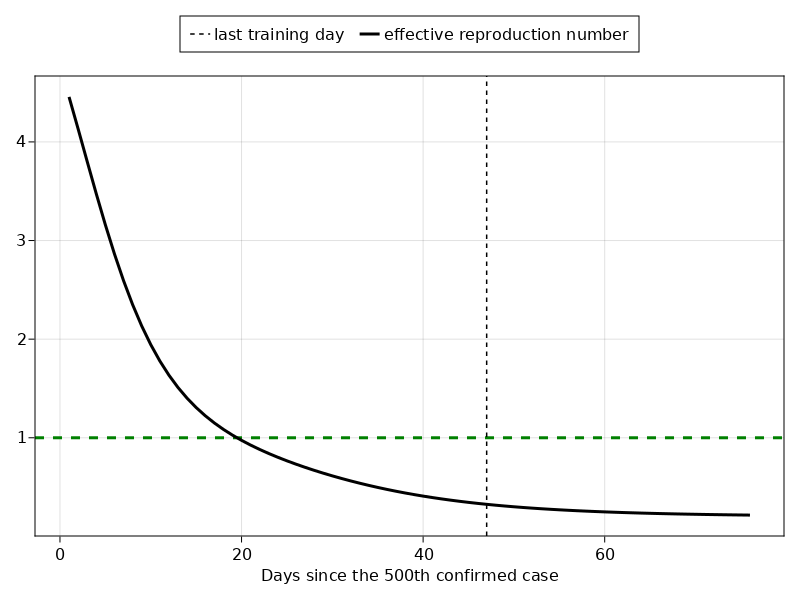
\includegraphics[width=\linewidth]{baseline/vietnam/20211216111951.baseline.vietnam.R_effective.png}
        \end{subfigure}
        \begin{subfigure}[b]{0.4\linewidth}
            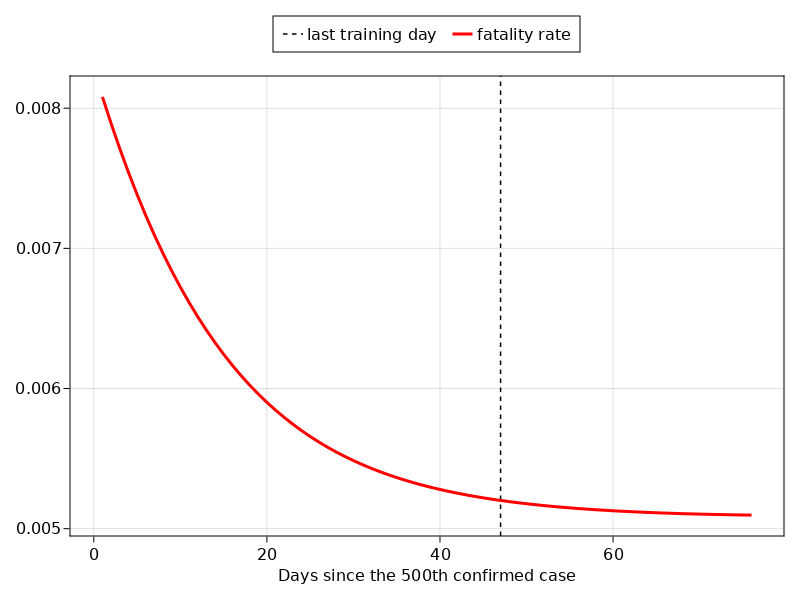
\includegraphics[width=\linewidth]{baseline/vietnam/20211216111951.baseline.vietnam.fatality_rate.png}
        \end{subfigure}
        \subcaption{Baseline model}
    \end{subfigure}

    \begin{subfigure}[b]{\linewidth}
        \centering
        \begin{subfigure}[b]{0.4\linewidth}
            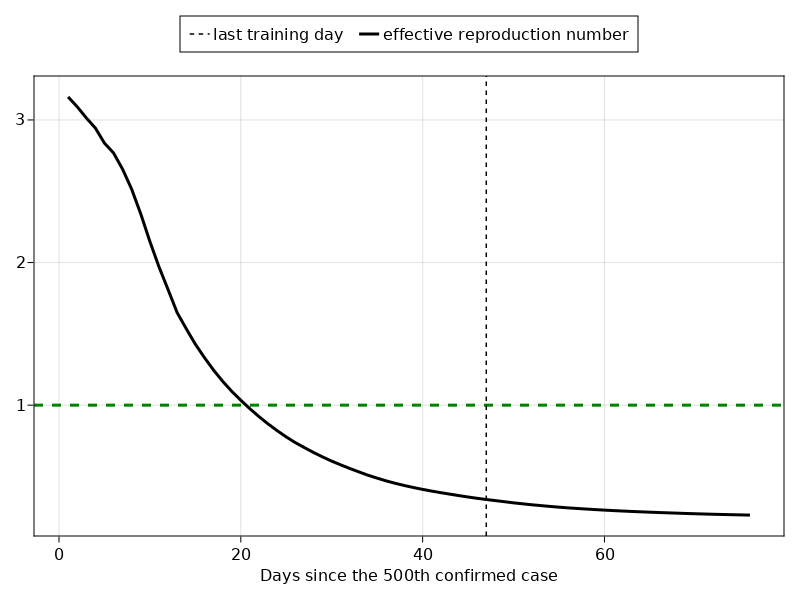
\includegraphics[width=\linewidth]{fb1/vietnam/20211216231719.fbmobility1.vietnam.R_effective.png}
        \end{subfigure}
        \begin{subfigure}[b]{0.4\linewidth}
            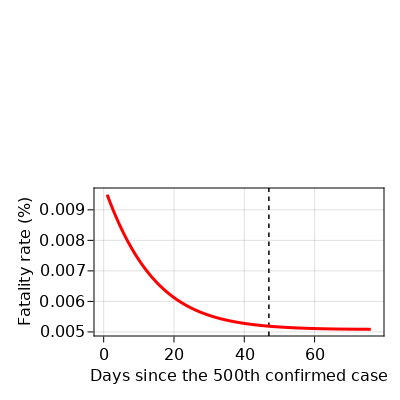
\includegraphics[width=\linewidth]{fb1/vietnam/20211216231719.fbmobility1.vietnam.fatality_rate.png}
        \end{subfigure}
        \subcaption{2nd. version}
    \end{subfigure}

    \caption{The effective reproduction number and the fatality rate for Vietnam learned by different versions of the model}
    \label{fig:R0-and-fatality-vietnam}
\end{figure}

\begin{figure}[!htb]
    \centering

    \begin{subfigure}[b]{\linewidth}
        \centering
        \begin{subfigure}[b]{0.4\linewidth}
            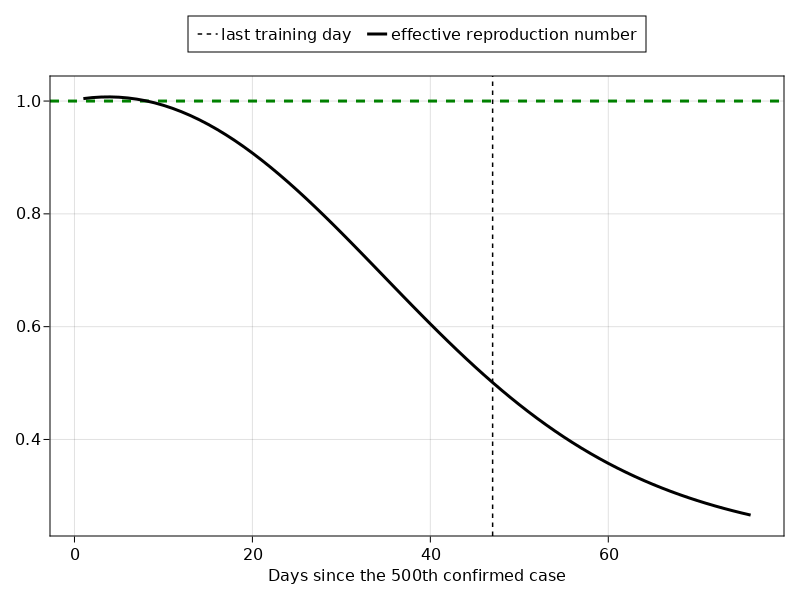
\includegraphics[width=\linewidth]{baseline/unitedstates/20211216125000.baseline.unitedstates.R_effective.png}
        \end{subfigure}
        \begin{subfigure}[b]{0.4\linewidth}
            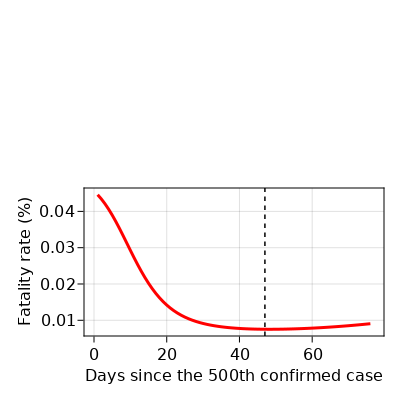
\includegraphics[width=\linewidth]{baseline/unitedstates/20211216125000.baseline.unitedstates.fatality_rate.png}
        \end{subfigure}
        \subcaption{Baseline model}
    \end{subfigure}

    \begin{subfigure}[b]{\linewidth}
        \centering
        \begin{subfigure}[b]{0.4\linewidth}
            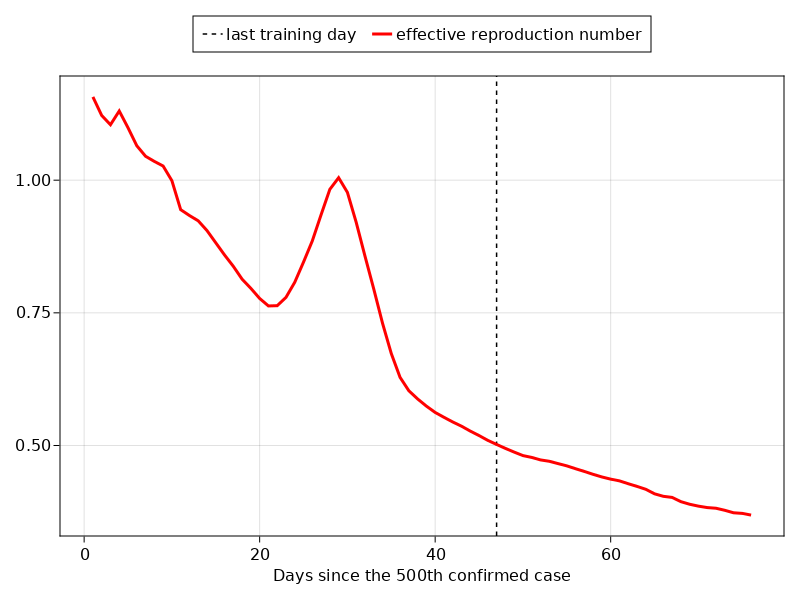
\includegraphics[width=\linewidth]{fb1/unitedstates/20211216233634.fbmobility1.unitedstates.R_effective.png}
        \end{subfigure}
        \begin{subfigure}[b]{0.4\linewidth}
            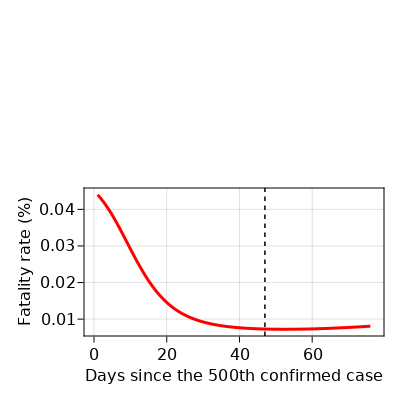
\includegraphics[width=\linewidth]{fb1/unitedstates/20211216233634.fbmobility1.unitedstates.fatality_rate.png}
        \end{subfigure}
        \subcaption{2nd. version}
    \end{subfigure}

    \caption{The effective reproduction number and the fatality rate for the United States learned by different versions of the model}
    \label{fig:R0-and-fatality-usa}
\end{figure}
